\begin{center}
    %%%%%%%%%%%%%%%%%%%%%%%%%%%%%%%%%
    %%%%%%%% Samar's %%%%%%%%
    %%%%%%%%%%%%%%%%%%%%%%%%%%%%%%%%%
    \begin{tcolorbox}[colback=white, colframe=black, width=\textwidth, arc=6pt, boxrule=1pt]
        \sectiontitle{Enhanced Integrated Nuclear Systems for Transmutation and Efficient Isolation of Nuclides}
        \sectioncontent{
            Cyclus modules are being developed to represent XDS technologies and evaluate their impact on the U.S.
            spent nuclear fuel inventory. STANDARDS 5.0.1 is integrated to provide isotopic compositions and material streams.

            \vspace{1em}

            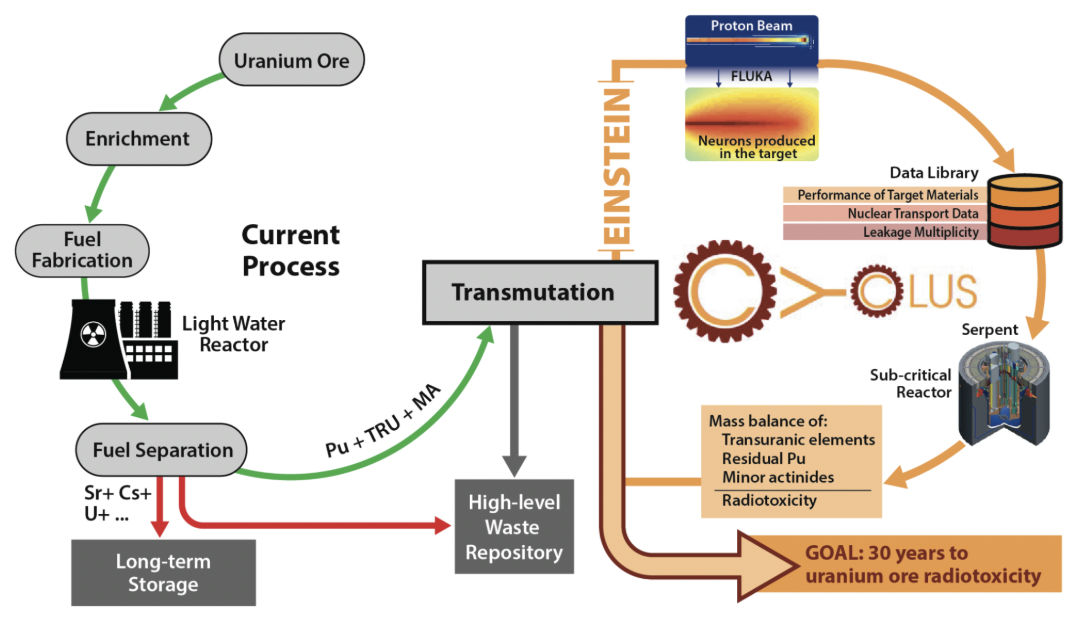
\includegraphics[width = 0.9\textwidth]{img/samar1.png}
            \figcaption{ARPAE EINSTEIN project \cite{fang_einstein_2025}.}
        }
    \end{tcolorbox}

    %%%%%%%%%%%%%%%%%%%%%%%%%%%%%%%%%
    %%%%%%%%%% Liam's %%%%%%%%%%
    %%%%%%%%%%%%%%%%%%%%%%%%%%%%%%%%%
    \begin{tcolorbox}[colback=white, colframe=black, width=\textwidth, arc=6pt, boxrule=1pt]
        \sectiontitle{RCANA}
        \sectioncontent{
            How can method of characteristics and computer graphics be implemented together to improve neutron transport?
            \par\vspace{1em}

           \begin{minipage}{.3\textwidth}
                \vspace{1em}
                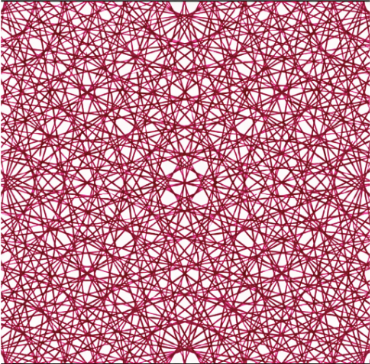
\includegraphics[width = \textwidth]{img/liam1.png}
                \newline
                \figcaption{
                    Method of Characteristics ray laydown example.
                }
            \end{minipage}
            \hspace{0.5cm}
            \begin{minipage}{.3\textwidth}
                \vspace{1em}
                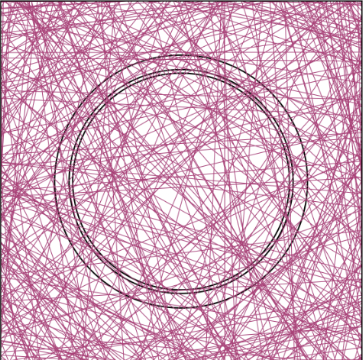
\includegraphics[width = \textwidth]{img/liam2.png}
                \newline
                \figcaption{
                    Random Ray laydown example \cite{trammRandomRayMethod2017a}.
                }
            \end{minipage}
            \hspace{0.5cm}
            \begin{minipage}{.3\textwidth}
                \vspace{1em}
                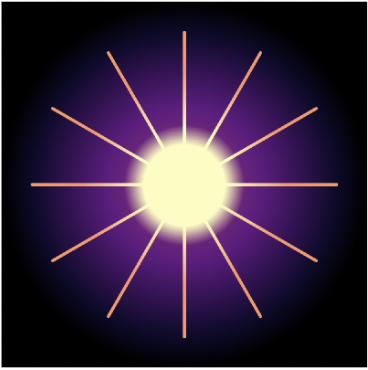
\includegraphics[width = \textwidth]{img/liam3.png}
                \newline
                \figcaption{
                    Future Innovations forthcoming.
                }
            \end{minipage}
        }
    \end{tcolorbox}


    %%%%%%%%%%%%%%%%%%%%%%%%%%%%%%%%%
    %%%%%%%%%%%%% HALEU %%%%%%%%%%%%%
    %%%%%%%%%%%%%%%%%%%%%%%%%%%%%%%%%
    \begin{tcolorbox}[colback=white, colframe=black, width=\textwidth, arc=6pt, boxrule=1pt]
        \sectiontitle{HALEU Studies}
        \sectioncontent{
            Investigating how uranium impurities in downblended highly enriched uranium (HEU) affect the performance and safety of high-temperature gas-cooled reactors (HTGRs).\\
            High-fidelity depletion simulations evaluate the impact of recycled fuel sources such as EBR-II and Y-12 on reactor behavior.
            

            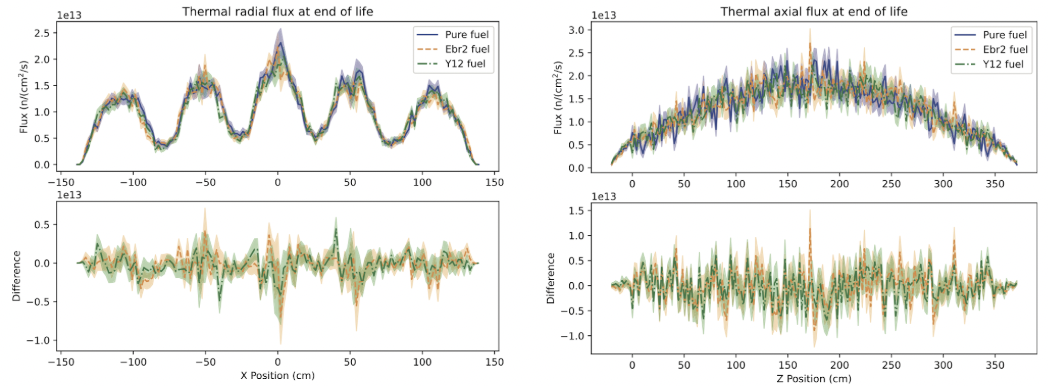
\includegraphics[width = 1.0\textwidth]{img/haleu.png}
            \newline
            \figcaption{
                Radial and axial thermal flux in the MMR-like reactor.
            }
        }
    \end{tcolorbox}

    %%%%%%%%%%%%%%%%%%%%%%%%%%%%%%%%%

\end{center}